%! Author = wolfram_e_laube
%! Date = 06.05.24

\item[(c)]
Below is the Python code for this exercise:

\begin{verbatim}
import matplotlib.pyplot as plt

# Set up frequency range
fs = 8e3  # Sampling frequency
frequencies = [1e3, fs - 1e3]  # Example frequencies
weights = [1, 0.5]  # Example weights

# Plot spectrum
plt.figure()
for f, w in zip(frequencies, weights):
    plt.arrow(f / 1e3, 0, 0, w, head_width=0.2, head_length=0.05, color='blue', length_includes_head=True)
    plt.arrow(-f / 1e3, 0, 0, w, head_width=0.2, head_length=0.05, color='blue', length_includes_head=True)

plt.xlim(-20, 20)
plt.xlabel('Frequency (kHz)')
plt.ylabel('Weight')
plt.title('Qualitative Spectrum of $x(t)$')
plt.grid(True)
plt.show()
\end{verbatim}

\begin{figure}[h]
    \centering
    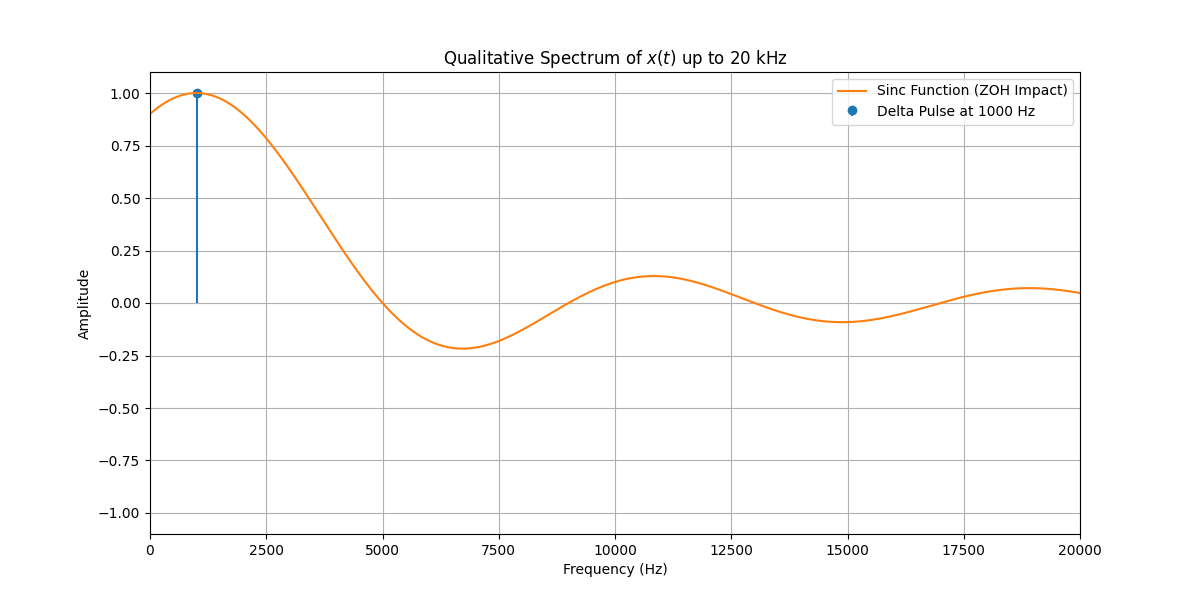
\includegraphics[width=0.49\textwidth]{fig/ex3_c_plot}
    \caption{Qualitative Spectrum of \(x(t)\)}
    \label{fig:ex3_c_plot}
\end{figure}
